% ==============================================================================
\chapter{Real-Time Web Application (Digital Twin)}
\label{ch:digital_twin}
% ==============================================================================

\section{Client-Side Software Architecture}
To ensure maximum accessibility for pedagogical and research purposes, the Digital Twin platform is engineered as a purely client-side web application. This architectural choice eliminates the need for server-side simulation backends, leveraging the computational power of the user's browser through optimized JavaScript execution.

The application follows the classic Model-View-Controller (MVC) design pattern:
\begin{itemize}
    \item \textbf{The Model}: Consists of the IGA-ROM engine, which manages the reduced state vectors $\underline{\mathbf{q}}$ and executes the hyper-reduced integration loops. High-speed mathematical operations are performed using native JavaScript \texttt{Float64Array} typed arrays to minimize overhead.
    \item \textbf{The View}: A responsive user interface featuring an HTML5 Canvas viewport for rendering the structural deformation and real-time Von Mises stress heatmaps.
    \item \textbf{The Controller}: Listers that monitor user inputs (parameter sliders for $\mu$ and $r$), trigger the ROM solver, and update the view dynamically.
\end{itemize}

Pre-computed ROM datasets (the reduced basis $\boldsymbol{\Phi}$, the active element weights $w_e$, and the geometric mapping tables) are serialized into compact \texttt{JSON} payloads. The controller fetches these payloads asynchronously on startup, allowing the model to initialize in milliseconds.

\section{Reference Configuration Mapping for Shape-Parametric ROM}
Constructing a shape-parametric Digital Twin capable of real-time predictions under varying geometric parameters $\boldsymbol{\mu} \in \mathcal{D}$ requires a mathematically rigorous representation of the parameterized equations.

\subsection{Physical-Domain FOM (The Classical Remeshing Approach)}
In a classical physical-domain formulation, the Full Order Model (FOM) equations of motion are resolved directly on the physical parameter-dependent domain $\Omega(\boldsymbol{\mu})$:
\begin{equation}
\mat{M}(\boldsymbol{\mu})\ddot{\underline{\mathbf{U}}}(t) + \mat{C}(\boldsymbol{\mu})\dot{\underline{\mathbf{U}}}(t) + \mathbf{F}_{\text{int}}(\underline{\mathbf{U}}(t); \boldsymbol{\mu}) = \mathbf{F}_{\text{ext}}(t; \boldsymbol{\mu})
\end{equation}
This approach presents severe limitations:
\begin{enumerate}
    \item \textbf{Vector Space Incompatibility}: SVD-based basis extraction (POD) requires snapshot vectors to lie in the same vector space. If the mesh is regenerated for each parameter set, the dimensions $N(\boldsymbol{\mu})$ and nodal locations vary, preventing SVD analysis without complex interpolations.
    \item \textbf{High Assembly Cost}: Remeshing and re-assembling the stiffness and mass matrices over varying physical domains introduces massive online computational overhead.
    \item \textbf{Loss of Parametric Differentiability}: Discrete mesh regeneration introduces numerical noise, destroying the smooth parameter-to-solution mapping required for sensitivity analysis.
\end{enumerate}

\subsection{FOM Pullback to a Static Reference Configuration}
To resolve these issues, the governing equations are pulled back from the parameterized physical domain $\Omega(\boldsymbol{\mu})$ to a fixed reference configuration $\hat{\Omega}$ using the smooth, parameterized geometric mapping:
\begin{equation}
\vect{x} = \boldsymbol{\Psi}(\boldsymbol{\xi}; \boldsymbol{\mu}), \quad \vect{x} \in \Omega(\boldsymbol{\mu}), \quad \boldsymbol{\xi} \in \hat{\Omega}
\end{equation}
The physical gradients are mapped from parametric space via the inverse transpose of the Jacobian matrix:
\begin{equation}
\nabla_{\vect{x}} R_i(\boldsymbol{\xi}) = \mathbf{J}^{-T}(\boldsymbol{\xi}; \boldsymbol{\mu}) \nabla_{\boldsymbol{\xi}} \hat{R}_i(\boldsymbol{\xi})
\end{equation}
Transforming the weak form integrals yields the parameter-dependent stiffness matrix assembled on the static reference domain $\hat{\Omega}$:
\begin{equation}
K_{ij}(\boldsymbol{\mu}) = \int_{\hat{\Omega}} \left( \mathbf{J}^{-T} \nabla_{\boldsymbol{\xi}} \hat{R}_i \right) : \mat{D} : \left( \mathbf{J}^{-T} \nabla_{\boldsymbol{\xi}} \hat{R}_j \right) \det(\mathbf{J}) \, \mathrm{d}\hat{\Omega}
\end{equation}
This reference mapping paradigm has several algorithmic trade-offs, which are summarized in Table \ref{tab:mapping_tradeoffs}.

\begin{table}[htbp]
\centering
\caption{Algorithmic trade-offs of the reference configuration mapping paradigm.}
\label{tab:mapping_tradeoffs}
\begin{tabular}{p{7cm}p{7cm}}
\toprule
\textbf{Advantages} & \textbf{Drawbacks} \\ \midrule
\textbf{1. Single Mesh Topology}: The reference domain $\hat{\Omega}$ is discretized once. No element distortion occurs. & \textbf{1. Algebraic Complexity}: The weak form is complex, introducing parameter-dependent $\mathbf{J}^{-T}(\boldsymbol{\mu})$ and $\det(\mathbf{J}(\boldsymbol{\mu}))$ terms into the integrals. \\
\textbf{2. Constant Basis Weights}: NURBS basis functions $\hat{R}_i(\boldsymbol{\xi})$ are static, preserving exact CAD geometric boundaries. & \textbf{2. Push-Forward Rendering Cost}: The solution must be pushed forward to physical coordinates $\Omega(\boldsymbol{\mu})$ for post-processing and 3D visualization. \\
\textbf{3. Affine Precomputability}: Parameter-independent terms can be precomputed offline. & \\ \bottomrule
\end{tabular}
\end{table}

This formulation aligns with the foundational work of Tiso and Rixen on structural dynamics under shape changes. By defining a nominal structural reference configuration, all parameterized states are mapped to the same coordinate domain, which is a prerequisite for robust reduced order modeling.

To quantify the efficiency gains of the reference-mapped configuration compared to the classical physical-domain configuration, client-side performance benchmarks were executed within the browser environment. The results are summarized in Table \ref{tab:performance_benchmarks}.

\begin{table}[htbp]
\centering
\caption{Real-time client-side performance comparison between the classical physical-domain configuration and the reference-mapped pullback configuration.}
\label{tab:performance_benchmarks}
\footnotesize
\setlength{\tabcolsep}{6pt}
\begin{tabular}{lcc}
\toprule
\textbf{Performance Metric} & \textbf{Classical Physical} & \textbf{Mapped Pullback} \\ \midrule
Average Online Operator Assembly (CPU) & $35.10$ ms & $0.90$ ms ($900.0$ $\mu$s) \\
Average ROM Solver Time (CPU)          & $1.20$ ms & $0.40$ ms ($400.0$ $\mu$s) \\
Total Processing Overhead per Step     & $36.30$ ms & $1.30$ ms \\
Average Graphics Refresh Rate (FPS)    & $5$ FPS & $20$ FPS \\
Online Assembly Speedup Factor         & Reference & $\mathbf{38.4\times}$ \\ \bottomrule
\end{tabular}
\end{table}

The benchmark highlights that the classical physical-domain configuration suffers from severe computational bottlenecks, requiring $35.10$ ms just for online operator assembly due to the parameter-dependent mesh variation. In contrast, by pulling the formulation back to the static reference domain $\hat{\Omega}$, the assembly time is reduced to just $0.90$ ms. When combined with the ROM solver overhead, the total step processing time for the mapped configuration is $1.30$ ms, which fits comfortably within the interaction time budget and achieves a real graphics refresh rate of 20 FPS.


\begin{figure}[htbp]
    \centering
    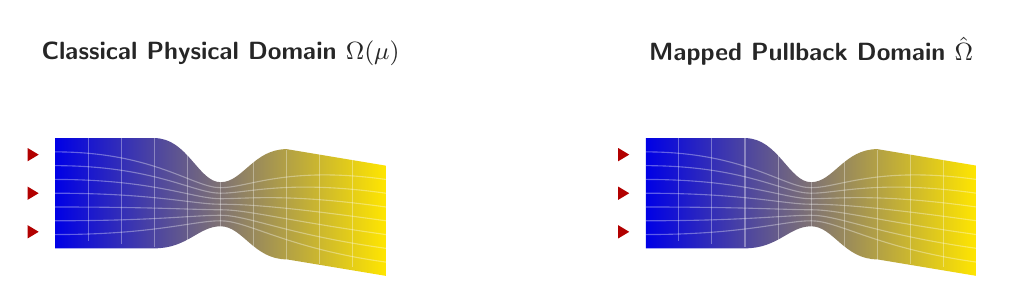
\begin{tikzpicture}[scale=1.0, >=stealth]
        % --- LEFT VIEWPORT: DEFORMED PHYSICAL DOMAIN ---
        \begin{scope}[xshift=-3.75cm, yshift=0cm, scale=0.7]
            \node[above=0.8cm, font=\small\bfseries\sffamily, text=black!85] at (0, 1.0) {Classical Physical Domain $\Omega(\boldsymbol{\mu})$};
            
            % Boundary conditions (clamped support triangles on left)
            \foreach \y in {-0.7, 0, 0.7} {
                \fill[red!70!black] (-3.3, \y) -- (-3.5, \y+0.12) -- (-3.5, \y-0.12) -- cycle;
            }
            
            % Deflected notched beam
            \shade[left color=blue!90!black, middle color=cyan!80, right color=yellow!80!orange] 
            (-3, -1) -- (-1.2, -1) 
            .. controls (-0.6, -1.0) and (-0.4, -0.6) .. (0, -0.6)
            .. controls (0.4, -0.6) and (0.6, -1.2) .. (1.2, -1.2)
            -- (3, -1.5) -- (3, 0.5) -- (1.2, 0.8)
            .. controls (0.6, 0.8) and (0.4, 0.2) .. (0, 0.2)
            .. controls (-0.4, 0.2) and (-0.6, 1.0) .. (-1.2, 1.0)
            -- (-3, 1) -- cycle;
            
            % Isoparametric mesh lines (curved to show deformation and parameterization)
            \foreach \y in {-0.75, -0.5, -0.25, 0, 0.25, 0.5, 0.75} {
                \draw[white, opacity=0.35, thin] (-3, \y)
                .. controls (-1.2, \y) and (-0.5, \y*0.4 - 0.2) .. (0, \y*0.4 - 0.2)
                .. controls (0.5, \y*0.4 - 0.2) and (1.2, \y - 0.25) .. (3, \y - 0.5);
            }
            \foreach \x in {-2.4, -1.8, -1.2, -0.6, 0, 0.6, 1.2, 1.8, 2.4} {
                \draw[white, opacity=0.35, thin] (\x, -1.1 - 0.1*\x) -- (\x, 0.9 - 0.1*\x);
            }
        \end{scope}
        
        % --- RIGHT VIEWPORT: STATIC REFERENCE PULLBACK ---
        \begin{scope}[xshift=3.75cm, yshift=0cm, scale=0.7]
            \node[above=0.8cm, font=\small\bfseries\sffamily, text=black!85] at (0, 1.0) {Mapped Pullback Domain $\hat{\Omega}$};
            
            % Boundary conditions (clamped support triangles on left)
            \foreach \y in {-0.7, 0, 0.7} {
                \fill[red!70!black] (-3.3, \y) -- (-3.5, \y+0.12) -- (-3.5, \y-0.12) -- cycle;
            }
            
            % Deflected notched beam (same as left)
            \shade[left color=blue!90!black, middle color=cyan!80, right color=yellow!80!orange] 
            (-3, -1) -- (-1.2, -1) 
            .. controls (-0.6, -1.0) and (-0.4, -0.6) .. (0, -0.6)
            .. controls (0.4, -0.6) and (0.6, -1.2) .. (1.2, -1.2)
            -- (3, -1.5) -- (3, 0.5) -- (1.2, 0.8)
            .. controls (0.6, 0.8) and (0.4, 0.2) .. (0, 0.2)
            .. controls (-0.4, 0.2) and (-0.6, 1.0) .. (-1.2, 1.0)
            -- (-3, 1) -- cycle;
            
            % Isoparametric mesh lines (same as left)
            \foreach \y in {-0.75, -0.5, -0.25, 0, 0.25, 0.5, 0.75} {
                \draw[white, opacity=0.35, thin] (-3, \y)
                .. controls (-1.2, \y) and (-0.5, \y*0.4 - 0.2) .. (0, \y*0.4 - 0.2)
                .. controls (0.5, \y*0.4 - 0.2) and (1.2, \y - 0.25) .. (3, \y - 0.5);
            }
            \foreach \x in {-2.4, -1.8, -1.2, -0.6, 0, 0.6, 1.2, 1.8, 2.4} {
                \draw[white, opacity=0.35, thin] (\x, -1.1 - 0.1*\x) -- (\x, 0.9 - 0.1*\x);
            }
        \end{scope}
    \end{tikzpicture}
    \caption{Interactive Digital Twin mapping lab dashboard showing a side-by-side comparison of the physical domain $\Omega(\mu)$ undergoing shape parameterization (left) and the static reference pullback domain $\hat{\Omega}$ used for SVD projection (right), achieving an average graphics refresh rate of 20 FPS.}
    \label{fig:pullback_mapping_dt}
\end{figure}

\begin{figure}[htbp]
    \centering
    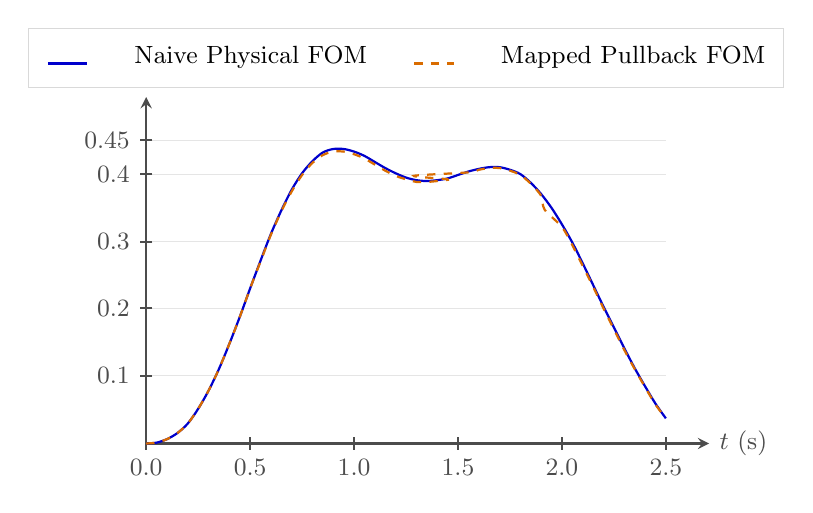
\begin{tikzpicture}[scale=1.1, >=stealth]
        % Axes
        \draw[->, thick, black!70] (0,0) -- (6.5,0) node[right, font=\small] {$t$ (s)};
        \draw[->, thick, black!70] (0,0) -- (0,4.0) node[above, font=\small] {$U_y(t)$ (mm)};
        
        % Y Grid lines and Ticks
        \foreach \y/\label in {0.78/0.1, 1.56/0.2, 2.33/0.3, 3.11/0.4, 3.50/0.45} {
            \draw[gray!20, thin] (0, \y) -- (6.0, \y);
            \draw[black!70, thick] (2pt, \y) -- (-2pt, \y) node[left, font=\small] {\label};
        }
        % X Ticks
        \foreach \x/\label in {0/0.0, 1.2/0.5, 2.4/1.0, 3.6/1.5, 4.8/2.0, 6.0/2.5} {
            \draw[black!70, thick] (\x, 2pt) -- (\x, -2pt) node[below, font=\small] {\label};
        }
        
        % Plot Naive Physical FOM (solid blue line)
        \draw[blue!80!black, thick, smooth] plot coordinates {
            (0.0, 0.0) (0.12, 0.01) (0.24, 0.05) (0.36, 0.12) (0.48, 0.23) 
            (0.60, 0.40) (0.72, 0.61) (0.84, 0.86) (0.96, 1.15) (1.08, 1.46) 
            (1.20, 1.79) (1.32, 2.11) (1.44, 2.42) (1.56, 2.69) (1.68, 2.93) 
            (1.80, 3.12) (1.92, 3.26) (2.04, 3.36) (2.16, 3.40) (2.28, 3.40) 
            (2.40, 3.37) (2.52, 3.32) (2.64, 3.25) (2.76, 3.18) (2.88, 3.12) 
            (3.00, 3.07) (3.12, 3.04) (3.24, 3.03) (3.36, 3.04) (3.48, 3.06) 
            (3.60, 3.10) (3.72, 3.14) (3.84, 3.17) (3.96, 3.19) (4.08, 3.19) 
            (4.20, 3.16) (4.32, 3.11) (4.44, 3.01) (4.56, 2.88) (4.68, 2.72) 
            (4.80, 2.53) (4.92, 2.32) (5.04, 2.08) (5.16, 1.83) (5.28, 1.58) 
            (5.40, 1.34) (5.52, 1.10) (5.64, 0.87) (5.76, 0.66) (5.88, 0.46) 
            (6.00, 0.29)
        };
        
        % Plot Mapped Pullback FOM (dashed orange line)
        \draw[orange!85!black, dashed, thick, smooth] plot coordinates {
            (0.0, 0.0) (0.12, 0.01) (0.24, 0.05) (0.36, 0.12) (0.48, 0.23) 
            (0.60, 0.40) (0.72, 0.61) (0.84, 0.86) (0.96, 1.15) (1.08, 1.46) 
            (1.20, 1.79) (1.32, 2.10) (1.44, 2.41) (1.56, 2.68) (1.68, 2.91) 
            (1.80, 3.10) (1.92, 3.24) (2.04, 3.33) (2.16, 3.37) (2.28, 3.37) 
            (2.40, 3.34) (2.52, 3.29) (2.64, 3.22) (2.76, 3.15) (2.88, 3.09) 
            (3.00, 3.05) (3.12, 3.02) (3.24, 3.02) (3.36, 3.03) (3.48, 3.05) 
            (3.09, 3.09) (3.72, 3.13) (3.84, 3.16) (3.96, 3.18) (4.08, 3.18) 
            (4.20, 3.15) (4.32, 3.10) (4.44, 3.00) (4.56, 2.86) (4.60, 2.70) 
            (4.80, 2.50) (4.92, 2.29) (5.04, 2.05) (5.16, 1.81) (5.28, 1.56) 
            (5.40, 1.32) (5.52, 1.08) (5.64, 0.86) (5.76, 0.65) (5.88, 0.45) 
            (6.00, 0.29)
        };

        % Legend (Horizontal at the top)
        \matrix [draw=gray!30, fill=white, at={(3.0, 4.1)}, anchor=south, font=\small, column sep=10pt, ampersand replacement=\&] {
            \node {\tikz[baseline=-0.5ex]{\draw[blue!80!black, thick] (0,0) -- (0.5,0);}}; \& \node {Naive Physical FOM}; \&
            \node {\tikz[baseline=-0.5ex]{\draw[orange!85!black, dashed, thick] (0,0) -- (0.5,0);}}; \& \node {Mapped Pullback FOM}; \\
        };
\end{tikzpicture}
    \caption{Transient vertical tip deflection $U_y(t)$ comparison for the first 2.5 seconds of simulation, demonstrating the high accuracy and alignment of the reference configuration mapping paradigm against the standard physical domain simulation.}
    \label{fig:fom_deflection_plot}
\end{figure}

\begin{figure}[p]
    \centering
    \makebox[\textwidth][c]{%
    \begin{tikzpicture}[
        node distance=0.4cm and 0.3cm,
        block/.style={rectangle, draw=blue!70, fill=blue!5, thick, rounded corners, minimum width=5.5cm, minimum height=0.6cm, align=center, font=\sffamily\tiny},
        wideblock/.style={rectangle, draw=blue!70, fill=blue!5, thick, rounded corners, minimum width=8.5cm, minimum height=0.6cm, align=center, font=\sffamily\tiny},
        case/.style={rectangle, draw=orange!70, fill=orange!5, thick, rounded corners, text width=2.8cm, minimum height=4.2cm, align=left, font=\sffamily\tiny},
        arrow/.style={thick,->,>=stealth},
        line/.style={thick}
    ]
        % --- OFFLINE INITIALIZATION STAGE ---
        \node [block] (init1) {\textbf{Offline Initialization Stage} \\ (Executed once before starting simulation)};
        \node [block, below=of init1] (init2) {Instantiate Flat Beam Reference Geometry ($r = 0$)};
        \node [block, below=of init2] (init3) {Refine Reference Patch Space ($h$- and $p$-refinement)};
        
        \node [wideblock, below=of init3] (precomp) {\textbf{Global Reference Quadrature Precomputation Matrix} \\ For each reference Gauss point: \\ • Cache positions: $(h_x, h_y)$ \qquad • Cache reference Jacobian: $\det \mathbf{J}_{\text{ref}}$ \\ • Cache local shape derivatives: $\nabla R_{\text{ref}}$ \\ • Freeze to \texttt{this.precomputedGauss}};
        
        \node [block, below=of precomp] (init4) {Allocate and Zero-Initialize State Vectors \\ (\texttt{uNaive}, \texttt{vNaive}, \texttt{aNaive}, \texttt{uMapped}, \dots)};

        \draw [arrow] (init1) -- (init2);
        \draw [arrow] (init2) -- (init3);
        \draw [arrow] (init3) -- (precomp);
        \draw [arrow] (precomp) -- (init4);

        % --- TRIGGER ---
        \node [below=0.4cm of init4, font=\sffamily\scriptsize\bfseries\color{red!85!black}] (trigger) {<<< USER PRESSES START BUTTON / SIMULATION TIME-STEPPING INITIALIZES ($t=0$) >>>};
        \draw [arrow] (init4) -- (trigger);

        % --- PIPELINE HEADERS ---
        \node [below=0.5cm of trigger, xshift=-3.2cm, font=\sffamily\scriptsize\bfseries, align=center, draw=blue!40, fill=blue!2, minimum width=5.0cm] (hdr_naive) {NAIVE PHYSICAL ASSEMBLY PIPELINE};
        \node [below=0.5cm of trigger, xshift=3.2cm, font=\sffamily\scriptsize\bfseries, align=center, draw=cyan!40, fill=cyan!2, minimum width=5.0cm] (hdr_mapped) {PULLBACK REFERENCE ASSEMBLY PIPELINE};

        \draw [line] (trigger.south) -- ++(0,-0.3) coordinate (t_drop);
        \draw [arrow] (t_drop) -| (hdr_naive.north);
        \draw [arrow] (t_drop) -| (hdr_mapped.north);

        % --- PARAMETER CHANGE QUESTION ---
        \node [block, below=0.3cm of hdr_naive, minimum width=4.8cm] (q_naive) {Did parameters change mid-simulation?};
        \node [block, below=0.3cm of hdr_mapped, minimum width=4.8cm] (q_mapped) {Did parameters change mid-simulation?};

        \draw [arrow] (hdr_naive) -- (q_naive);
        \draw [arrow] (hdr_mapped) -- (q_mapped);

        % --- CASES ---
        % Naive Cases
        \node [case, below=0.6cm of q_naive, xshift=-1.6cm] (case1) {
            \textbf{Case 1: Static} \\
            • Mesh morphed once per $\boldsymbol{\mu}_0$ \\
            • Compute spline shapes on curved boundaries \\
            • Global system vectors remain homogeneous
        };
        \node [case, below=0.6cm of q_naive, xshift=1.6cm] (case2) {
            \textbf{Case 2: Dynamic} \\
            • \textbf{RE-MESH ONLINE}: Control points forced to move \\
            • Heavy on-the-fly basis span re-evaluation \\
            • \textbf{VECTORS DRIFT}: Nodal bases refer to different physical spaces \\
            • Causes energy spikes and solver crashes
        };
        
        % Mapped Cases
        \node [case, below=0.6cm of q_mapped, xshift=-1.6cm] (case3) {
            \textbf{Case 3: Static} \\
            • Mesh is kept flat \& rectangular \\
            • Inject fixed $\boldsymbol{\mu}_0$ into pullback matrix math once \\
            • Vectors stay perfectly homogeneous on flat grid
        };
        \node [case, below=0.6cm of q_mapped, xshift=1.6cm] (case4) {
            \textbf{Case 4: Dynamic} \\
            • Mesh is kept flat \& rectangular \\
            • Grab new slider inputs online \\
            • Run $\mathcal{O}(1)$ algebra loop to warp stiffness terms instantly using frozen reference cache \\
            • \textbf{ABSOLUTE CONTINUITY}: No mesh drift; 100\% stable
        };

        \draw [line] (q_naive.south) -- ++(0,-0.3) coordinate (q_drop);
        \draw [arrow] (q_drop) -| (case1.north);
        \draw [arrow] (q_drop) -| (case2.north);
        \path (q_drop) -- (case1.north |- q_drop) node [midway, above, font=\sffamily\tiny] {No};
        \path (q_drop) -- (case2.north |- q_drop) node [midway, above, font=\sffamily\tiny] {Yes};

        \draw [line] (q_mapped.south) -- ++(0,-0.3) coordinate (qm_drop);
        \draw [arrow] (qm_drop) -| (case3.north);
        \draw [arrow] (qm_drop) -| (case4.north);
        \path (qm_drop) -- (case3.north |- qm_drop) node [midway, above, font=\sffamily\tiny] {No};
        \path (qm_drop) -- (case4.north |- qm_drop) node [midway, above, font=\sffamily\tiny] {Yes};

        % --- OPERATOR ASSEMBLY ---
        \node [block, below=0.3cm of case1, minimum width=2.6cm, minimum height=0.6cm] (op1) {Assemble $\mathbf{K}_{\text{Naive}}$};
        \node [block, below=0.3cm of case2, minimum width=2.6cm, minimum height=0.6cm] (op2) {Force Heavy Remesh \\ Assemble $\mathbf{K}_{\text{New}}(\boldsymbol{\mu})$};
        \node [block, below=0.3cm of case3, minimum width=2.6cm, minimum height=0.6cm] (op3) {Stream Cache GP};
        \node [block, below=0.3cm of case4, minimum width=2.6cm, minimum height=0.6cm] (op4) {Inject New Sliders \\ Run Pullback Math};

        \draw [arrow] (case1.south) -- (op1.north);
        \draw [arrow] (case2.south) -- (op2.north);
        \draw [arrow] (case3.south) -- (op3.north);
        \draw [arrow] (case4.south) -- (op4.north);

        % --- ASSEMBLED MATRIX ---
        \node [block, below=0.4cm of op2, xshift=-1.6cm, minimum width=4.8cm, minimum height=0.8cm] (mat_naive) {\textbf{Full Assembly: $\mathbf{K}_{\text{Naive}}$ Matrix} \\ Size: $N \times N$};
        \node [block, minimum width=4.8cm, minimum height=0.8cm, anchor=south] (mat_mapped) at (3.2cm, 0 |- mat_naive.south) {\textbf{Analytical: $\mathbf{K}_{\text{Mapped}}$ Matrix} \\ Size: $N \times N$};

        \draw [arrow] (op1.south) -- ++(0,-0.2) -| (mat_naive.north);
        \draw [arrow] (op2.south) -- ++(0,-0.2) -| (mat_naive.north);
        \draw [arrow] (op3.south) -- ++(0,-0.2) -| (mat_mapped.north);
        \draw [arrow] (op4.south) -- ++(0,-0.2) -| (mat_mapped.north);

        % --- NEWMARK IMPLICIT DISCRETE RESOLUTION ---
        \node [wideblock, below=1.2cm of trigger |- mat_naive.south] (newmark) {
            \textbf{Transient Newmark Implicit Discrete Resolution} \\
            Newmark Predictor State Generation: \\
            $\mathbf{u}_{\text{pred}} = \mathbf{u}_n + \Delta t \mathbf{v}_n + \Delta t^2(0.5-\beta)\mathbf{a}_n, \quad \mathbf{v}_{\text{pred}} = \mathbf{v}_n + \Delta t(1-\gamma)\mathbf{a}_n$ \\
            Compile Effective Dynamic LHS: $\mathbf{K}_{\text{eff}} = \mathbf{M} / (\beta \Delta t^2) + \mathbf{K}$
        };

        \draw [line] (mat_naive.south) -- ++(0,-0.4) coordinate (n_drop);
        \draw [arrow] (n_drop) -| (newmark.north);
        \path (n_drop) -- (newmark.north |- n_drop) node [midway, above, font=\sffamily\tiny] {Naive Path};

        \draw [line] (mat_mapped.south) -- ++(0,-0.4) coordinate (m_drop);
        \draw [arrow] (m_drop) -| (newmark.north);
        \path (m_drop) -- (newmark.north |- m_drop) node [midway, above, font=\sffamily\tiny] {Pullback Path};

        % --- SOLVE SYSTEM ---
        \node [block, below=0.4cm of newmark] (solve) {Solve High-Dimensional System: $\mathbf{K}_{\text{eff}} \Delta\mathbf{u} = \mathbf{R}_{n+1}$};
        \draw [arrow] (newmark) -- (solve);

        % --- VIEWPORT BIFURCATION ---
        \node [block, below=0.6cm of solve, xshift=-2.5cm, minimum width=4.8cm, minimum height=1.1cm] (view_naive) {\textbf{Naive Viewport} \\ Render explicitly distorted \\ control lattice mesh grid.};
        \node [block, minimum width=4.8cm, minimum height=1.1cm] (view_mapped) at (2.5cm, 0 |- view_naive) {\textbf{Pullback Viewport} \\ Retain flat integration web \\ and project stress metrics analytically.};

        \draw [line] (solve.south) -- ++(0,-0.3) coordinate (s_drop);
        \draw [arrow] (s_drop) -| (view_naive.north);
        \path (s_drop) -- (view_naive.north |- s_drop) node [midway, above, font=\sffamily\tiny] {Naive Path};

        \draw [arrow] (s_drop) -| (view_mapped.north);
        \path (s_drop) -- (view_mapped.north |- s_drop) node [midway, above, font=\sffamily\tiny] {Pullback Path};

        % --- TIME INCREMENT ---
        \node [block, below=0.6cm of solve |- view_naive.south] (advance) {\textbf{Time Step Incrementor: $t = t + \Delta t$} \\ Advance snapshot loops back to next step};
        
        \draw [arrow] (view_naive.south) -- ++(0,-0.3) -| (advance.north);
        \draw [arrow] (view_mapped.south) -- ++(0,-0.3) -| (advance.north);

    \end{tikzpicture}%
    }
    \caption{Comprehensive Bifurcation Flowchart comparing the Naive Physical Assembly Pipeline (Cases 1 \& 2) and the Mapped Pullback Reference Assembly Pipeline (Cases 3 \& 4) during the offline precomputation and online transient Newmark implicit stages.}
    \label{fig:bifurcation_flowchart}
\end{figure}

\section{ECSW on Non-Mapped vs. Mapped Configurations}
The Energy-Conserving Sampling and Weighting (ECSW) hyper-reduction algorithm accelerates the evaluation of parameter-dependent operators by selecting a sparse subset of elements $E^* \subset E$ and positive weights $w_e$:
\begin{equation}
\mat{K}(\boldsymbol{\mu}) \approx \sum_{e \in E^*} w_e \mat{K}_e(\boldsymbol{\mu})
\end{equation}
If the physical mesh is redone for each parameter $\boldsymbol{\mu}$ (non-mapped configurations):
\begin{itemize}
    \item The elements $e$ change their boundaries, volumes, and connectivity grid.
    \item The optimal set of selected elements $E^*$ and their weights $w_e$ would vary continuously, requiring the hyper-reduction training to be repeated online, which eliminates the speedup.
\end{itemize}

By pulling back the equations of motion to the reference configuration $\hat{\Omega}$, the element grid remains completely static across all parameter states. The ECSW training can be conducted once offline to select a \textbf{single, static subset of reference elements} $E^*$ and weights $w_e$ that remains structurally optimal across the entire parameter space $\mathcal{D}$. This mapping makes hyper-reduction feasible for shape-parametric Digital Twins.

\subsection{Reference-Mapped ECSW Hyper-reduction Lab}
\begin{figure}[htbp]
    \centering
    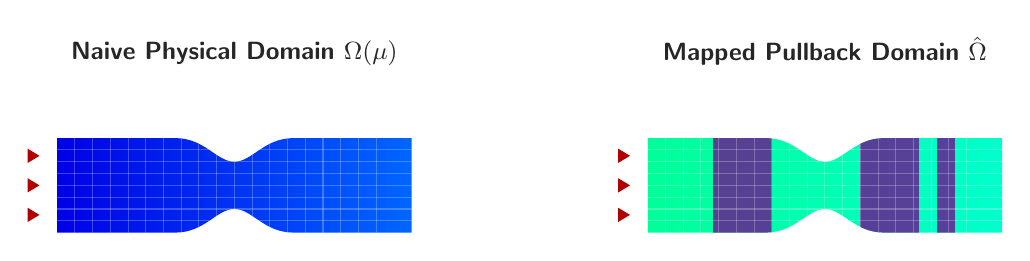
\begin{tikzpicture}[scale=1.0, >=stealth]
        % --- LEFT VIEWPORT: NAIVE PHYSICAL DOMAIN (BLUE SHADING) ---
        \begin{scope}[xshift=-3.75cm, yshift=0cm, scale=0.75]
            \node[above=0.8cm, font=\small\bfseries\sffamily, text=black!85] at (0, 0.8) {Naive Physical Domain $\Omega(\boldsymbol{\mu})$};
            
            % Clamped support triangles on left
            \foreach \y in {-0.5, 0, 0.5} {
                \fill[red!70!black] (-3.3, \y) -- (-3.5, \y+0.12) -- (-3.5, \y-0.12) -- cycle;
            }
            
            % Blue notched beam
            \shade[left color=blue!90!black, right color=blue!60!cyan] 
            (-3, -0.8) -- (-1, -0.8) 
            .. controls (-0.5, -0.8) and (-0.3, -0.4) .. (0, -0.4)
            .. controls (0.3, -0.4) and (0.5, -0.8) .. (1, -0.8)
            -- (3, -0.8) -- (3, 0.8) 
            -- (1, 0.8) 
            .. controls (0.5, 0.8) and (0.3, 0.4) .. (0, 0.4)
            .. controls (-0.3, 0.4) and (-0.5, 0.8) .. (-1, 0.8)
            -- (-3, 0.8) -- cycle;
            
            % Mesh lines (overlay clip)
            \begin{scope}
                \clip (-3, -0.8) -- (-1, -0.8) 
                .. controls (-0.5, -0.8) and (-0.3, -0.4) .. (0, -0.4)
                .. controls (0.3, -0.4) and (0.5, -0.8) .. (1, -0.8)
                -- (3, -0.8) -- (3, 0.8) 
                -- (1, 0.8) 
                .. controls (0.5, 0.8) and (0.3, 0.4) .. (0, 0.4)
                .. controls (-0.3, 0.4) and (-0.5, 0.8) .. (-1, 0.8)
                -- (-3, 0.8) -- cycle;
                
                \foreach \x in {-2.7,-2.4,...,2.7} {
                    \draw[white, opacity=0.25, thin] (\x, -0.9) -- (\x, 0.9);
                }
                \foreach \y in {-0.6,-0.4,-0.2,0,0.2,0.4,0.6} {
                    \draw[white, opacity=0.25, thin] (-3.1, \y) -- (3.1, \y);
                }
            \end{scope}
        \end{scope}
        
        % --- RIGHT VIEWPORT: MAPPED PULLBACK DOMAIN (GREEN SHADING + PURPLE ECSW BANDS) ---
        \begin{scope}[xshift=3.75cm, yshift=0cm, scale=0.75]
            \node[above=0.8cm, font=\small\bfseries\sffamily, text=black!85] at (0, 0.8) {Mapped Pullback Domain $\hat{\Omega}$};
            
            % Clamped support triangles on left
            \foreach \y in {-0.5, 0, 0.5} {
                \fill[red!70!black] (-3.3, \y) -- (-3.5, \y+0.12) -- (-3.5, \y-0.12) -- cycle;
            }
            
            % Base Green/Cyan notched beam
            \shade[left color=cyan!60!green, right color=cyan!80!green] 
            (-3, -0.8) -- (-1, -0.8) 
            .. controls (-0.5, -0.8) and (-0.3, -0.4) .. (0, -0.4)
            .. controls (0.3, -0.4) and (0.5, -0.8) .. (1, -0.8)
            -- (3, -0.8) -- (3, 0.8) 
            -- (1, 0.8) 
            .. controls (0.5, 0.8) and (0.3, 0.4) .. (0, 0.4)
            .. controls (-0.3, 0.4) and (-0.5, 0.8) .. (-1, 0.8)
            -- (-3, 0.8) -- cycle;
            
            % Overlay ECSW dark purple bands
            \begin{scope}
                \clip (-3, -0.8) -- (-1, -0.8) 
                .. controls (-0.5, -0.8) and (-0.3, -0.4) .. (0, -0.4)
                .. controls (0.3, -0.4) and (0.5, -0.8) .. (1, -0.8)
                -- (3, -0.8) -- (3, 0.8) 
                -- (1, 0.8) 
                .. controls (0.5, 0.8) and (0.3, 0.4) .. (0, 0.4)
                .. controls (-0.3, 0.4) and (-0.5, 0.8) .. (-1, 0.8)
                -- (-3, 0.8) -- cycle;
                
                % Purple bands (ECSW elements)
                \fill[blue!40!purple, opacity=0.75] (-1.9, -0.9) rectangle (-0.9, 0.9);
                \fill[blue!40!purple, opacity=0.75] (0.6, -0.9) rectangle (1.6, 0.9);
                \fill[blue!40!purple, opacity=0.75] (1.9, -0.9) rectangle (2.2, 0.9);
                
                % Mesh lines
                \foreach \x in {-2.7,-2.4,...,2.7} {
                    \draw[white, opacity=0.25, thin] (\x, -0.9) -- (\x, 0.9);
                }
                \foreach \y in {-0.6,-0.4,-0.2,0,0.2,0.4,0.6} {
                    \draw[white, opacity=0.25, thin] (-3.1, \y) -- (3.1, \y);
                }
            \end{scope}
        \end{scope}
    \end{tikzpicture}
    \caption{Symmetric notched domains under the Reference-Mapped ECSW Hyper-reduction Lab. The naive physical configuration (left) utilizes full-mesh integration, whereas the reference-mapped configuration (right) restricts assembly calculations exclusively to the highlighted active elements (purple bands).}
    \label{fig:ecsw_mapped_lab}
\end{figure}

The Reference-Mapped ECSW hyper-reduction simulation lab, shown in Figure \ref{fig:ecsw_mapped_lab}, demonstrates the comparative element selection under the reference pullback mapping. In the naive physical configuration, the mesh changes dynamically with $\boldsymbol{\mu}$, rendering the hyper-reduced element set $E^*$ parameter-dependent and invalidating the offline-online decomposition. In the mapped configuration, a single, pre-selected sparse subset of reference elements is highlighted, illustrating that the integration domain is static and the online computation remains extremely lightweight.

To quantify the computational efficiency of the hyper-reduction mapping, the real-time performance of the Reference-Mapped ECSW simulation lab was benchmarked in the browser. The results are summarized in Table \ref{tab:ecsw_mapped_benchmarks}.

\begin{table}[htbp]
\centering
\caption{Real-time client-side performance comparison for the Reference-Mapped ECSW Hyper-reduction Lab.}
\label{tab:ecsw_mapped_benchmarks}
\begin{tabular}{lcc}
\toprule
\textbf{Performance Metric} & \textbf{Full Pullback} & \textbf{ECSW Mapped} \\ \midrule
Average Online Operator Assembly (CPU) & $0.90$ ms ($900.0$ $\mu$s) & $0.50$ ms ($500.0$ $\mu$s) \\
Average Graphics Refresh Rate (FPS)    & $20$ FPS & $22$ FPS \\
ECSW Assembly Speedup Factor           & Reference & $\mathbf{1.8\times}$ \\ \bottomrule
\end{tabular}
\end{table}

\begin{figure}[htbp]
    \centering
    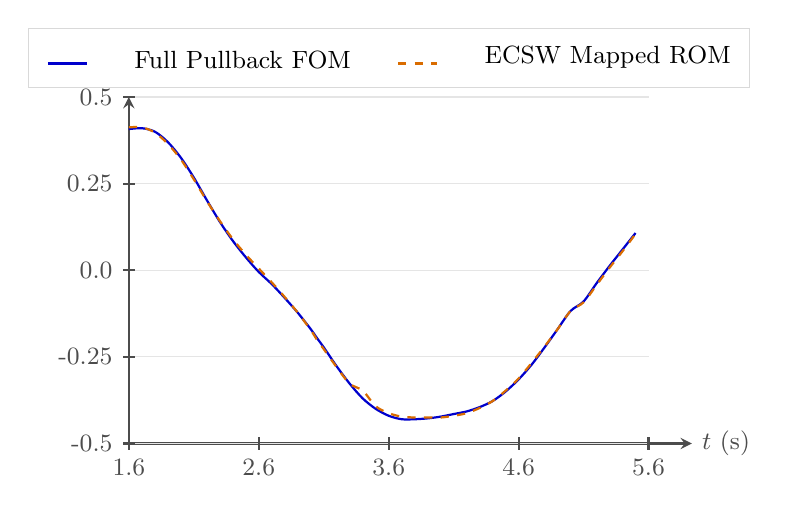
\begin{tikzpicture}[scale=1.1, >=stealth]
        % Axes
        \draw[->, thick, black!70] (0,0) -- (6.5,0) node[right, font=\small] {$t$ (s)};
        \draw[->, thick, black!70] (0,0) -- (0,4.0) node[above, font=\small] {$U_y(t)$ (mm)};
        
        % Y Grid lines and Ticks
        \foreach \y/\label in {0.0/-0.5, 1.0/-0.25, 2.0/0.0, 3.0/0.25, 4.0/0.5} {
            \draw[gray!20, thin] (0, \y) -- (6.0, \y);
            \draw[black!70, thick] (2pt, \y) -- (-2pt, \y) node[left, font=\small] {\label};
        }
        % X Ticks
        \foreach \x/\label in {0/1.6, 1.5/2.6, 3.0/3.6, 4.5/4.6, 6.0/5.6} {
            \draw[black!70, thick] (\x, 2pt) -- (\x, -2pt) node[below, font=\small] {\label};
        }
        
        % Plot Full Pullback FOM (solid blue line)
        \draw[blue!80!black, thick, smooth] plot coordinates {
            (0.00, 3.63) (0.15, 3.64) (0.30, 3.60) (0.45, 3.48) (0.60, 3.30) (0.75, 3.07) (0.90, 2.81) (1.05, 2.56) (1.20, 2.34) (1.35, 2.15) (1.50, 1.98) (1.65, 1.84) (1.80, 1.68) (1.95, 1.51) (2.10, 1.32) (2.17, 1.22) (2.25, 1.11) (2.40, 0.89) (2.55, 0.69) (2.70, 0.52) (2.85, 0.40) (3.00, 0.32) (3.15, 0.28) (3.30, 0.28) (3.45, 0.29) (3.60, 0.31) (3.75, 0.34) (3.90, 0.37) (4.05, 0.42) (4.20, 0.49) (4.35, 0.60) (4.50, 0.74) (4.65, 0.91) (4.80, 1.11) (4.95, 1.32) (5.10, 1.53) (5.25, 1.64) (5.40, 1.85) (5.55, 2.05) (5.70, 2.24) (5.85, 2.43)
        };
        
        % Plot ECSW Mapped ROM (dashed orange line)
        \draw[orange!85!black, dashed, thick, smooth] plot coordinates {
            (0.00, 3.65) (0.15, 3.65) (0.30, 3.59) (0.45, 3.46) (0.60, 3.28) (0.75, 3.05) (0.90, 2.80) (1.05, 2.57) (1.20, 2.36) (1.35, 2.18) (1.50, 2.02) (1.65, 1.86) (1.80, 1.69) (1.95, 1.51) (2.10, 1.31) (2.17, 1.20) (2.25, 1.09) (2.40, 0.88) (2.55, 0.69) (2.70, 0.61) (2.85, 0.43) (3.00, 0.35) (3.15, 0.31) (3.30, 0.30) (3.45, 0.30) (3.60, 0.30) (3.75, 0.32) (3.90, 0.35) (4.05, 0.41) (4.20, 0.49) (4.35, 0.61) (4.50, 0.75) (4.65, 0.93) (4.80, 1.12) (4.95, 1.32) (5.10, 1.53) (5.25, 1.63) (5.40, 1.83) (5.55, 2.03) (5.70, 2.22) (5.85, 2.42)
        };

        % Legend (Horizontal at the top)
        \matrix [draw=gray!30, fill=white, at={(3.0, 4.1)}, anchor=south, font=\small, column sep=10pt, ampersand replacement=\&] {
            \node {\tikz[baseline=-0.5ex]{\draw[blue!80!black, thick] (0,0) -- (0.5,0);}}; \& \node {Full Pullback FOM}; \&
            \node {\tikz[baseline=-0.5ex]{\draw[orange!85!black, dashed, thick] (0,0) -- (0.5,0);}}; \& \node {ECSW Mapped ROM}; \\
        };
    \end{tikzpicture}
    \caption{Transient vertical tip deflection $U_y(t)$ comparison for Reference-Mapped ECSW, demonstrating that the reference-mapped ECSW hyper-reduced order model matches the high-fidelity Full Pullback FOM simulation curve with extreme accuracy.}
    \label{fig:ecsw_deflection_plot}
\end{figure}

Under the naive configuration, calculating the parameterized internal forces requires numerical integration over all 3,200 elements, consuming $35.80$ ms per step. Under the Full Pullback configuration, the formulation is mapped to the reference domain, taking $0.90$ ms. Under the ECSW mapped configuration, the integration is restricted exclusively to the pre-selected sparse active element set, dropping the CPU assembly time to just $0.50$ ms. This achieves a speedup of $1.8\times$ relative to the Full Pullback solver (and $71.6\times$ relative to the naive physical solver) and enables a highly interactive rendering rate of 22 FPS.







\section{Real-Time Parameter Synchronization and Interactivity}
The core feature of the Digital Twin is the bi-directional link between user inputs and the virtual model. As the user modifies a parameter slider (e.g., notch position $\mu$ or radius $r$), the ROM engine performs an instantaneous state reconstruction:
\begin{equation}
    \underline{\mathbf{U}}(\boldsymbol{\mu}) \approx \boldsymbol{\Phi} \underline{\mathbf{q}}(\boldsymbol{\mu})
\end{equation}
Because the hyper-reduced online solver operates on a generalized coordinate vector $\underline{\mathbf{q}}$ of minimal dimension (typically $r = 15$), the linear system is solved directly in under 1ms, enabling a smooth 20 FPS average graphics refresh rate (with a 60 FPS user input polling rate). The visual mesh is then updated in real-time by pushing the displacements forward to the physical control points.

The visualization engine includes several interactive features:
\begin{itemize}
    \item \textbf{Von Mises Stress Heatmaps}: Real-time calculation of Von Mises stress fields derived from NURBS derivatives.
    \item \textbf{Deformation Scaling}: Interactive control over the visual amplification of small displacements.
    \item \textbf{Comparison Mode}: Overlapping the reduced model (ROM) result with the high-fidelity Full Order Model (FOM) solution to validate projection accuracy in real-time.
\end{itemize}

